\documentclass{article}
\usepackage[utf8]{inputenc}
\usepackage{graphicx}
\usepackage[breaklinks]{hyperref}
\usepackage{amsmath}
\usepackage{amssymb}

\begin{document}

\section{Slur control points}

We display slurs as two cubic Bézier curves, joined at the center point (thickest point of the slur).
In this document, we name the control points as follows (from left to right):
\begin{itemize}
\item $E_l$: left endpoint
\item $C_l$: point that controls the left corner shape
\item $S_l$: point that controls the pronouncedness of the left "shoulder"
\item $M$: midpoint (highest and thickest point, where both Bézier curves join)
\item $S_4$: point that controls the pronouncedness of the right "shoulder"
\item $C_r$: point that controls the right corner shape
\item $E_r$: right endpoint
\end{itemize}

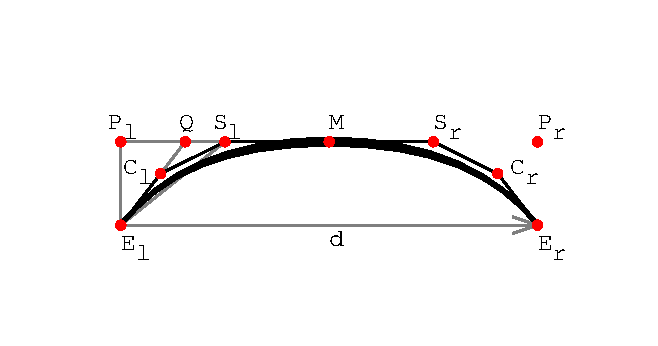
\includegraphics{slurCalcIllustration.eps}

This means we have seven points and therefore 14 degrees of freedom.
For a smooth transition between the to Bézier curves in point $M$, we will require $S_l M S_r$ to lie on a straight line
and the division ratios of $M P_r S_r$ and of $M P_l S_l$ to be equal.
This reduces the degrees of freedom to twelve, therefore we have to provide 12 parameters as follows:
\begin{itemize}
\item 4 parameters are given by specifying the endpoints
\item 2 parameters specify the position of the helper points $P_l$ and $P_r$
\item 1 parameter specifies the position of $M$
\item 1 parameter specifies the position of $S_l$ and $S_r$
\item 2$\cdot$2 parameters specify the tangent angle in the endpoints and the curvature
\end{itemize}

%This reduces the degrees of freedom to twelve, which means we need twelve parameters that define the final slur shape.

\section{Paremetrization}
\subsection{Endpoints $E_l$ and $E_r$}
The endpoints $E_l$ and $E_r$ are the most important parameters.
\subsection{Tilt $t$ and height $h$}
The tilt paramter $t$ and the height parameter $h$ define the positions of the two helper points $P_l$ and $P_r$.
Those two points are the reference points for calculating all other points.
For defining the four coordinates of the two points, we need two more conditions in addition to the two parameters $t$ and $h$.
So, we define that the lines $E_l P_l$ and $E_r P_r$ shall always be parallel, i.e. $\square E_l E_r P_r P_l$ always is a trapezoid.
\begin{equation}E_l P_l \parallel E_r P_r\end{equation}
Additionally, the angles $\angle P_l E_l E_r$ and $\angle P_r E_r E_l$ shall be right angles.
\begin{equation}E_l P_l \perp P_l P_r \end{equation}
((2) also implies $E_r P_r \perp P_l P_r$ because of (1).)

We define two special values for the tilt parameter $t$.
For $t=1$, the tangent in the thickest point shall be parallel to the base line $E_l E_r$.
For $t=0$, the tangent in the thickest point shall be horizontal.
We achieve this by defining the direction vector of the parallel vectors $\overrightarrow{E_l P_l}$ and $\overrightarrow{E_r P_r}$ as being
\begin{equation}v=\begin{pmatrix}-td_y\\d_x\end{pmatrix}\end{equation}
where
$$\begin{pmatrix}d_x\\d_y\end{pmatrix}=\begin{pmatrix}E_r - E_l\end{pmatrix}$$
Like this, $v$ is perpendicular to $\overrightarrow{E_l E_r}$ for $t=1$
(and because of (2) $\overrightarrow{E_l E_r}$ and $\overrightarrow{P_l P_r}$ are parallel).
For $t=0$, $v$ is vertical (and because of (2), $\overrightarrow{P_l P_r}$ is horizontal).
For convenience, we introduce the normalized unit vector belonging to $v$
$$\hat{v}=\frac{v}{||v||}$$

For $t=1$, $||E_l P_l||=:h_l$ and $||E_r P_r||=:h_r$ shall be equal to $h$, the height of the slur.
This means,
$$\begin{matrix}
P_l(t=1)=E_l + h\hat{v}&\\
P_r(t=1)=E_r + h\hat{v}&.
\end{matrix}$$
For $t\ne 1$, the two lengths can obviously not be equal, but we require their arithmetic mean to be equal to $h$.
This can be achieved by adding the same value $c$ to one length and subtract it from the other.
This value is somehow dependent on $t$ (for $t=1$ it's 0).
\begin{equation}\begin{matrix}
h_l=h+c(t) \\
h_r=h-c(t)
\end{matrix}\end{equation}
We need $h_l$ and $h_r$ to calculate $P_l$ and $P_r$:
$$\begin{matrix}
P_l=E_l+h_l\hat{v}\\
P_r=E_r+h_r\hat{v}
\end{matrix}$$

Using condition (2), we derive a calculation rule for $c(t)$ via the standard dot product of $v$ and $\overrightarrow{P_l P_r}$,
which is required to be 0 as condition (2) demands the two vectors to be perpendicular.

\begin{eqnarray*}
\langle P_r-P_l, v\rangle &=& \langle [E_r+h_r\hat{v}]-[E_l+h_l\hat{v}],v\rangle\\
&=& \langle [E_r+(h-c(t))\hat{v}]-[E_l+(h+c(t))\hat{v}],v\rangle\\
&=& \langle [E_r-E_l] + [(h-c(t))-(h+c(t))]\hat{v},v\rangle\\
&=& \langle \begin{pmatrix}d_x\\d_y\end{pmatrix} + [-2c(t)]\frac{v}{||v||},v\rangle\\
&=& \langle \begin{pmatrix}d_x\\d_y\end{pmatrix} - \frac{2c(t)}{||v||}\begin{pmatrix}-td_y\\d_x\end{pmatrix},\begin{pmatrix}-td_y\\d_x\end{pmatrix}\rangle\\
&=& (d_x+\frac{2c(t)}{||v||}td_y)(-td_y)+(d_y-\frac{2c(t)}{||v||}d_x)d_x\\
&=& -d_xtd_y-\frac{2c(t)}{||v||}t^2d_y^2+d_yd_x-\frac{2c(t)}{||v||}d_x^2\\
&=& d_xd_y(1-t)-\frac{2c(t)}{||v||}(t^2d_y^2+d^2)\\
&\stackrel{t^2d_y^2+d^2=||v||^2}{=}& d_xd_y(1-t)-2c(t)||v||\\
&\stackrel{!}{=}&0\\
\Rightarrow c(t)&=& \frac{(1-t)d_xd_y}{2||v||}
\end{eqnarray*}

Now we can calculate $P_l$ and $P_r$ as follows:
\begin{eqnarray}\begin{matrix}
P_l=E_l+h_l\hat v=E_l+(h+c(t))\hat v\\
P_r=E_r+h_r\hat v=E_r+(h-c(t))\hat v
\end{matrix}\end{eqnarray}

\subsection{Shift $f$ of the midpoint $M$}
The midpoint's position between $P_l$ and $P_r$ is defined by its "shift" $f$.
$f$ makes the midpoint travel along an imaginry rail that goes from $P_l$ to $P_r$.
For $f=0$ it's centered between $P_l$ and $P_r$, 
for $f=-1$, $M$ falls together with $P_l$ and for $f=1$ it falls together with $P_r$.
The formula for M is
$$M=P_l+\frac{f+1}{2}(P_r - P_l)$$

\subsection{Shoulder parameter $s$ and shoulder points $S_l$ and $S_r$}
The "shoulder" parameter $s$ defines the position of the Bézier control points $S_l$ and $S_r$.
This parameter should take on values between 0 and 1 and moves the $E$ points 
further to the center or further to the sides.
$s=0$ means that the slur's shoulder is minmal and the shoulder points move to the center,
i.e. $S_l = S_r = M$.
$s=1$ means that the shoulder is as pronounced as possible, i.e. $S_l=P_l$ and $S_r=P_r$.
The formula for $S_l$ is
$$S_l=M+s(P_l-M) $$
and $S_r$ works analogously.

As a smooth transition between the two Bézier curves is desired we're using the same $s$ on both sides.
The most widely used method to make the transition look smooth is to make $S_l$ and $S_r$ symmetric with 
$M$ as point of symmetry (i.e. $M - S_l = S_r - M$, compare e.g.
\href{http://www.w3.org/TR/SVG/paths.html#PathDataCubicBezierCommands}{SVG's smooth curve commands}).
We're not using this method because it doesn't work well for asymmetric slurs.
This method only guarantees mathematically strict continuity of curvature at $M$ 
in the symmetry case, anyway. Our method guarantees this as well.

\subsection{Endpoint angle $a$}
The parameters $a_l$ and $a_r$ define the tangents in the slur's endpoints.
(The tangents could be controlled individually for each side using $a_l$ and $a_r$,
or by a parameter $a$ that controls both sides.)
The tangents are the lines $E_l Q_l$ and $E_r Q_r$.
$Q_l$ and $Q_r$ are usually located on the line segments $\overline{P_l S_l}$ and $\overline{P_r S_r}$.
If they were closer to $M$, the control polygons would not be concave any more. If they were further outside, the slur would get
"potbellys" that are protruding over the edges $E_l$ and $E_r$.

$Q_l$ and $Q_r$ are calculated in the same way as $S_l$ and $S_r$:
$$Q_l=S_l+a_l(P_l-S_l)$$
(analogously for $Q_r$).
This means, for $a=0$ the slur shape starts/levels off as flat as possible and for $a=1$ it's as stepp as possible.

\subsection{Curvature parameters $c_l$ and $c_r$}
The parameters $c_l$ and $c_r$ fix the $C$ control points by describing their "height" over the line $E_l E_r$.
This can be thought of as influencing the curvature (therefore $c$).
With all other parameters set, $c=0$ makes the curvature minmial ("slow", wide curve)
and $c=1$ makes it maximal ("sharper" turn), while keeping the control polygon convex.
$C_l$ and $C_r$ are calculated in the familiar manner
$$C_l=E_l+c_l(Q_l-E_l)$$
(analogously for $C_r$).

\subsection{Thickness parameters $t_{min}$, $t_{max}$ and $w$}
The maximum thickness (in point $M$) is defined by the parameter $t_{max}$, the minimum thickness (in the endpoints) by parameter $t_{min}$.
How "fast" the slur gets thicker towards the center can be influenced with the swelling rate parameter $w$.
The swelling rate on the left and right sides could also be controlled individually by $w_l$ and $w_r$ parameters.
All those parameters are needed to calculate the actual control points for the slur outline as described below.

\section{Slur profile}
As slurs are thinner at the tips and thicker at the center, we need a "sandwich" of Bézier curves (two top and two bottom curves).
To achieve the profile, we use control points that--compared to the ones shown in the illustration--are offset slightly upwards or downwards.

$M$, $S_l$ and $S_r$ are offset by half of the desired width in the center--minus half of the desired width at the tips
as we're stroking the outlines to get rounded tips with a defined thickness.
How far the points $C_l$ and $C_r$ are offset is defined by parameter $w$.
For $w=1$, they are offset by the same vector as $M$, for $w=0$, they are not offset at all.

The offset vector for $M$, $S_l$ and $S_r$, which we call $o$, is calculated as follows:
$$o=(t_{max}-t_{min})\hat v$$
The offset vector for $S_l$ and $S_r$ is
\begin{eqnarray*}
o_l=w_lo\\
o_r=w_ro
\end{eqnarray*}

The sandwich consists of the following control points: On the top we have

$E_{l}$, $C_{tl}$, $S_{tl}$, $M_t$, $S_{tr}$, $C_{tr}$ and $E_{r}$.

On the bottom we have analogously

$E_{l}$, $C_{bl}$, $S_{bl}$, $M_b$, $S_{br}$, $C_{br}$ and $E_{r}$.

Those offset points on the left half are calculated as follows:
\begin{eqnarray*}
C_{tl}&=&C+wo\\
C_{bl}&=&C-wo\\
S_{tl}&=&S_l+o\\
S_{bl}&=&S_l-o\\
M_{t}&=&M+o\\
M_{b}&=&M-o
\end{eqnarray*}

\end{document}
